

%%
%% Algorithm
%%


\begin{frame}{Row Merge Algorithm}

\begin{center}
\only<1>{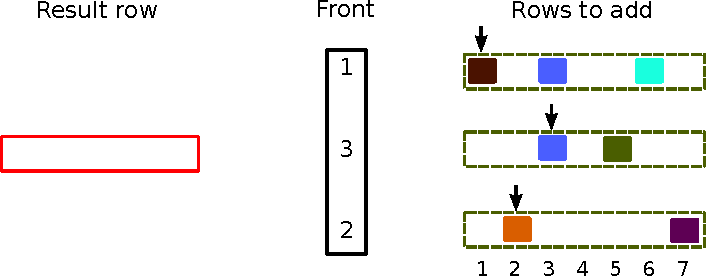
\includegraphics[width=0.7\textwidth]{figures/spgemm-row-0} }\only<2>{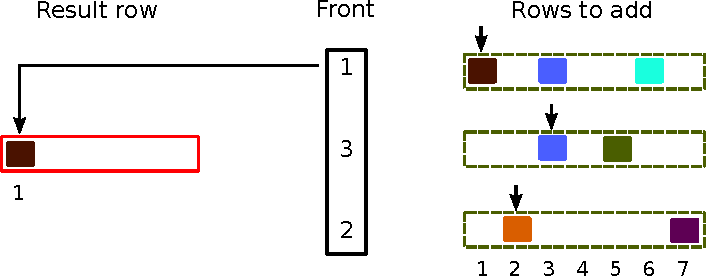
\includegraphics[width=0.7\textwidth]{figures/spgemm-row-1} }\only<3>{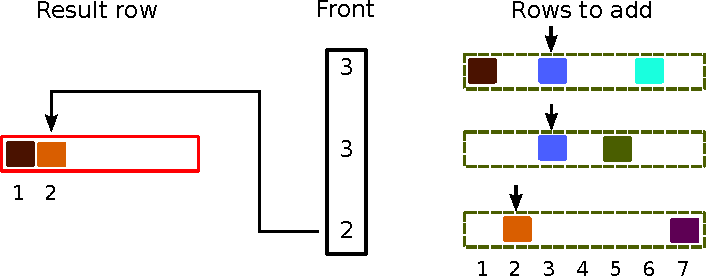
\includegraphics[width=0.7\textwidth]{figures/spgemm-row-2} }\only<4>{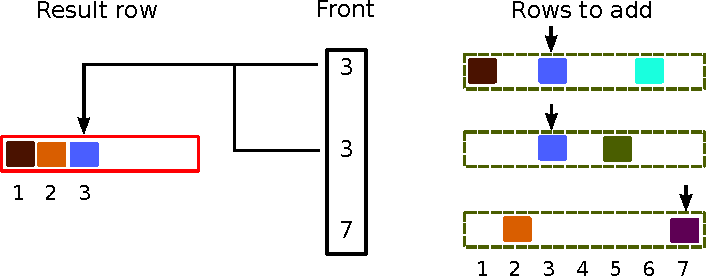
\includegraphics[width=0.7\textwidth]{figures/spgemm-row-3} }\only<5>{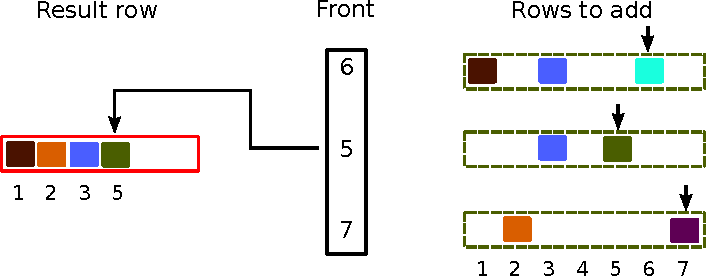
\includegraphics[width=0.7\textwidth]{figures/spgemm-row-4} }\only<6>{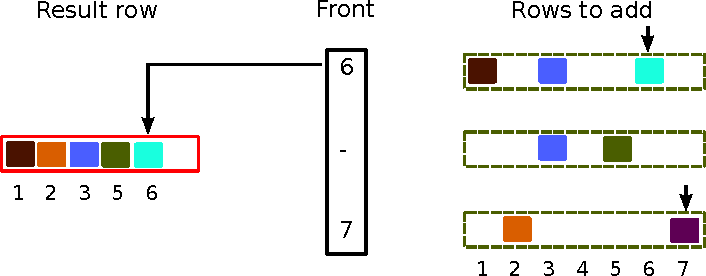
\includegraphics[width=0.7\textwidth]{figures/spgemm-row-5} }\only<7>{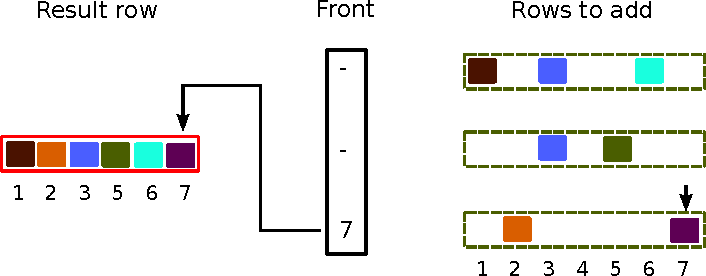
\includegraphics[width=0.7\textwidth]{figures/spgemm-row-6} }
\end{center}


\begin{block}{Result Row Computation}
 \begin{enumerate}
  \item Determine minimum index in front
  \pause
  \item Write minimum index
  \pause
  \item Advance front where minimum index occurred
 \end{enumerate}

\end{block}


\end{frame}

%%%%%%%%%%%


\begin{frame}[fragile]{Sparse Matrix Products}

 \begin{minipage}{0.44\textwidth}
 \begin{block}{Algorithm Details}
  \begin{itemize}
   \item Split matrix if rows too large
   \item Recursively merge 8 rows
   \item (Re-)use scratchpad memory
  \end{itemize}
 \end{block}
 \end{minipage}
 \begin{minipage}{0.55\textwidth}
  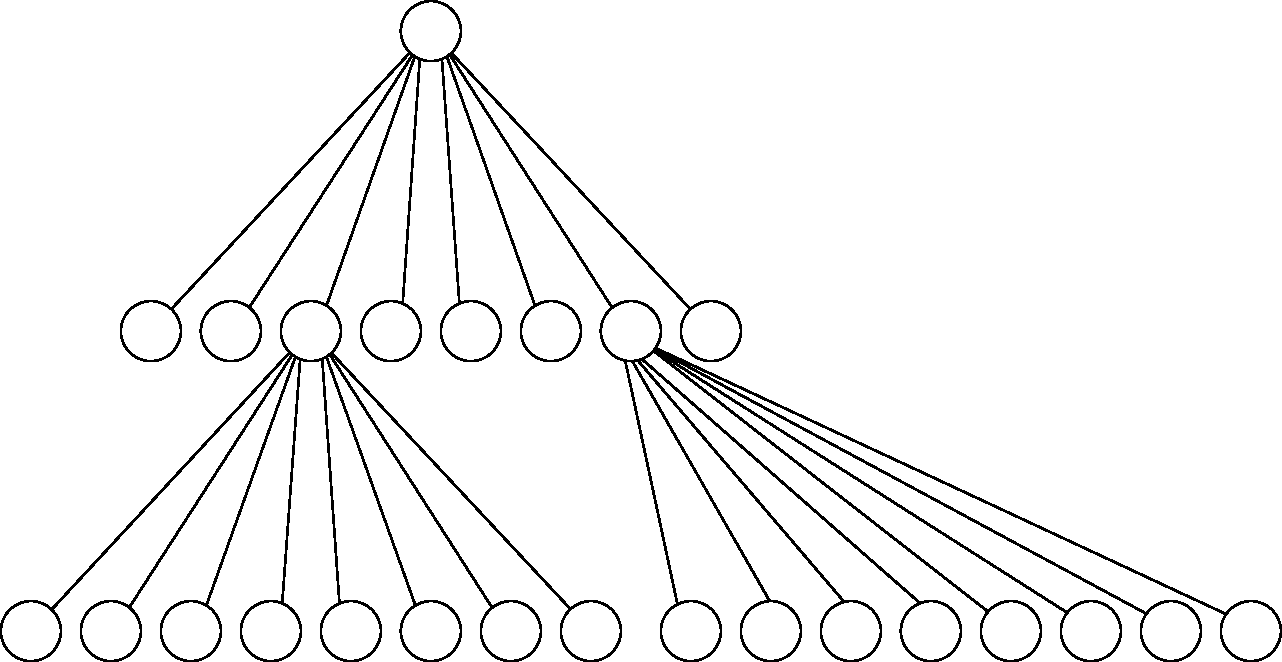
\includegraphics[width=0.999\textwidth]{figures/Octree2} \\
  {\tiny \verb|https://en.wikipedia.org/wiki/Octree\#/media/File:Octree2.svg|}
 \end{minipage}

 \pause
 \begin{block}{Hardware Details}
  \begin{itemize}
   \item CPU: Use AVX2 to merge 8 rows simultaneously
   \item GPU: Merge up to 32/64 rows simultaneously with one warp/wavefront
   \item MIC: Use AVX-KNC to merge 16 rows simultaneously
  \end{itemize}
 \end{block}

 \pause
  \begin{block}{Parallelization and Load Balancing}
  \begin{itemize}
   \item CPU, MIC: Use MPI!
   \item CPU, MIC, alternative: OpenMP dynamic scheduling, chunk size 1024
   \item GPU: thread scheduling in hardware
  \end{itemize}
 \end{block}


\end{frame}

